%%%%%%%%%%%%%%%%%%%%%%% file template.tex %%%%%%%%%%%%%%%%%%%%%%%%%
%
% This is a general template file for the LaTeX package SVJour3
% for Springer journals.          Springer Heidelberg 2010/09/16
%
% Copy it to a new file with a new name and use it as the basis
% for your article. Delete % signs as needed.
%
% This template includes a few options for different layouts and
% content for various journals. Please consult a previous issue of
% your journal as needed.
%
%%%%%%%%%%%%%%%%%%%%%%%%%%%%%%%%%%%%%%%%%%%%%%%%%%%%%%%%%%%%%%%%%%%
%
% First comes an example EPS file -- just ignore it and
% proceed on the \documentclass line
% your LaTeX will extract the file if required
\begin{filecontents*}{example.eps}
%!PS-Adobe-3.0 EPSF-3.0
%%BoundingBox: 19 19 221 221
%%CreationDate: Mon Sep 29 1997
%%Creator: programmed by hand (JK)
%%EndComments
gsave
newpath
  20 20 moveto
  20 220 lineto
  220 220 lineto
  220 20 lineto
closepath
2 setlinewidth
gsave
  .4 setgray fill
grestore
stroke
grestore
\end{filecontents*}
%
\RequirePackage{fix-cm}
%
%\documentclass{svjour3}                     % onecolumn (standard format)
%\documentclass[smallcondensed]{svjour3}     % onecolumn (ditto)
\documentclass[smallextended]{svjour3}       % onecolumn (second format)
%\documentclass[twocolumn]{svjour3}          % twocolumn
%
\smartqed  % flush right qed marks, e.g. at end of proof
%
\usepackage{graphicx}
\usepackage{todonotes}
%
% \usepackage{mathptmx}      % use Times fonts if available on your TeX system
%
% insert here the call for the packages your document requires
%\usepackage{latexsym}
% etc.
%
% please place your own definitions here and don't use \def but
% \newcommand{}{}
%
% Insert the name of "your journal" with
% \journalname{myjournal}
%
\begin{document}

\title{Insert your title here%\thanks{Grants or other notes
%about the article that should go on the front page should be
%placed here. General acknowledgments should be placed at the end of the article.}
}
\subtitle{Do you have a subtitle?\\ If so, write it here}

%\titlerunning{Short form of title}        % if too long for running head

\author{First Author         \and
        Second Author %etc.
}

%\authorrunning{Short form of author list} % if too long for running head

\institute{F. Author \at
              first address \\
              Tel.: +123-45-678910\\
              Fax: +123-45-678910\\
              \email{fauthor@example.com}           %  \\
%             \emph{Present address:} of F. Author  %  if needed
           \and
           S. Author \at
              second address
}

\date{Received: date / Accepted: date}
% The correct dates will be entered by the editor


\maketitle

\begin{abstract}
Insert your abstract here. Include keywords, PACS and mathematical
subject classification numbers as needed.
\keywords{First keyword \and Second keyword \and More}
% \PACS{PACS code1 \and PACS code2 \and more}
% \subclass{MSC code1 \and MSC code2 \and more}
\end{abstract}

\section{Introduction}
\label{sec:intro}

\begin{quote}
	In order to discover the actual steps by which the male of any existing 
	bird has acquired his magnificent colours or other ornaments, we ought 
	to behold the long line of his extinct progenitors; \emph{but this is obviously impossible}.\footnote{Emphasis ours.} \\
	\\
	--- Charles Darwin, in reference to peacocks~\cite{Darwin} 
\end{quote}

After people began to realize that species were not fixed, and that the fossil 
record contained evidence of a long and complex natural history, it also
became clear that this record was terribly incomplete. In the quote above
Darwin clearly realized the potential value of a complete ancestral record in
understanding evolutionary processes, but he also took it as a given that
such a record was not to be had.

The incompleteness of the historical record, both human and natural, continues
to challenge scholars in a host of fields. Paleontologists work with a 
profoundly
incomplete fossil record, often describing and classifying entire categories of
organisms based a few teeth. The human historical record is no more complete,
with numerous valuable resources lost to the ravages of time. Worse, these 
gaps are often neither random nor symmetric, substantially skewing our view 
of that history. Teeth, for example, are often all we have of ancient 
sharks and their kin because their skeletons are made of cartilage, which
typically doesn't fossilize, and the lives and ideas of people with wealth, 
power, and education are far more likely to be preserved than those of the
poor and illiterate.

While it was impossible for Darwin to ``behold the long line of \ldots 
[peacock] progenitors'', in evolutionary computation it is in principle possible
to save \emph{all} the data from a run, and indeed explore all the progenitors
of a successful individual. As described in Section~\ref{sec:EC_pattern},
however, we rarely collect and analyze this type of data, instead only sharing
thin statistically summaries, pale shadows of the extremely complex 
processes that stand behind our research. 
In this paper, however, we propose
saving far more data tha has been common in the field, recording all the ``little'' low-level events that ultimately drive whatever large-scale trends 
we observe in our runs. While the majority of EC research fails to record more
than a tiny fraction of this detail, there are exceptions, some of which 
will be discussed in Section~\ref{sec:related}.

Recording all these low-level events does represent a substantial increase 
in the amount of data
collected, which means that we need tools and techniques to store, explore,
analyze, and share results from that data. In recent work~\cite{graph_db_work}
we have found graph databases (discussed in
Section~\ref{sec:graph_DBs}) to be an effective tool for managing the 
substantial collection of data generated during a run. 

Visualizations are central to the success
of our work with graph databases, and Section~\ref{sec:visualizations}
describes our design of data rich 
visualizations that allow us to effectively explore and share results such as
complex ancestry graphs. We will then share examples of things we've learned
from such ancestry graphs in Section~\ref{sec:learned}, and present conclusions
and ideas for future work in Section~\ref{sec:conclusions}.

\section{A common pattern in EC research}
\label{sec:EC_pattern}

A common pattern in published evolutionary computation research is to
compare approach $A$ and approach $B$ (perhaps two different selection
mechanisms, or two different recombination operators) by doing a number
of runs with each approach, often on several different ``representative''
problems. Then a table of summary statistics is reported that (usually)
suggests that one of the two methods had some sort of advantage over
the other.

As an example, Table~\ref{tab:example_table} (which is a subset of a 
much larger dataset presented in \cite{Helmuth:Benchmarks}) presents
the number of successes out of 100 independent when comparing three
different selection mechanisms across a number of software synthesis
problems. The results in this table (which are supported and extended
in the full table) suggest that on this set of test problems lexicase
selection is generally the most successful.

\begin{table}
	% table caption is above the table
	\caption{An example of summary reseaerch results, taken from
	\cite{Helmuth:Benchmarks}. This shows the number of successes
    out of 100 independent runs on several software sythesis problems,
    for each of three selection mechanisms: Tournament, Implicit Fitness Sharing (IFS), and Lexicase. \underline{Underline} indicates a statistically
    significant advantage over both other selection methods at $p < 0.05$
    based on a pairwise chi-square test with Holm correction.}
	\label{tab:example_table}       % Give a unique label
	% For LaTeX tables use
	\begin{tabular}{llll}
		\hline\noalign{\smallskip}
		Problem & Tourn. & IFS & Lex. \\
		\noalign{\smallskip}\hline\noalign{\smallskip}
		Number IO & 68 & 72 & \underline{98} \\
		Smallest & 75 & \underline{98} & 81 \\
		String Lengths Backwards & 7 & 10 & \underline{66} \\
		Replace Space With Newline & 8 & 16 & \underline{51} \\
		Vector Average & 14 & 13 & 16 \\
		Small Or Large & 3 & 3 & 5 \\
		For Loop Index & 0 & 0 & 1 \\
		String Differences & 0 & 0 & 0 \\
		\noalign{\smallskip}\hline
	\end{tabular}
\end{table}

This is a useful result, and clearly tells us something valuable about
these three selection mechanisms in the tested domain. It also leaves
so much unsaid, however, about the \emph{why} of this result. It's great
to know that lexicase selection has a distinct and general advantage on 
these problems, but we have no idea \emph{why} lexicase selection is
outperforming the other two approaches. The handful of numbers in
Table~\ref{tab:example_table} are summarizing the complex ``lives'' 
and interactions of 100's of millions of individuals, but those numbers
tell us nothing about how those billions of micro-events add up to this
overall result. This is not simply a pedantic observation, as this lost 
information also represents a lost opportunity for greater understanding. 

We might, for example, see a similar table in the social sciences, 
perhaps listing economic metrics like gross domestic product for 
various countries. That might give us a high level view of the relationship
of those countries economies, but no one would claim to \emph{understand}
those relationships based on the table alone. Understanding would come
from unpacking that small set of numbers, and trying to describe the
mechanisms that underlie them. 

Yet published research in evolutionary
computation regularly ``ends'' with something like 
Table~\ref{tab:example_table}, with no empirically grounded discussion 
of the mechanisms that might lead to these summary results. The detailed
data about the events that drive these results aren't presented or discussed,
and likely aren't collected or even available to the researchers themselves.
It is extremely common in evolutionary computation research to effectively
throw away all that data as the runs progress\ldots
\todo[inline]{finish this paragraph}

\todo[inline]{Skim through GECCO papers counting number that have
this form?}

\section{Related work}
\label{sec:related}

We are not aware of any other work in evolutionary computation using graph
databases to store and analyze full ancestry trees in a systematic way. That
said, there is other work where ancestry information has been collected,
analyzed, and visualized.

\todo[inline]{Crib stuff from, e.g., the VizGEC paper in Denver.}

\section{Graph databases}
\label{sec:graph_DBs}

\section{Visualizations}
\label{sec:visualizations}

\section{What have we learned?}
\label{sec:learned}

\section{Conclusions}
\label{sec:conclusions}

\todo[inline]{We may want a separate future work section? Not sure.}

\section*{Random examples from Springer}

\todo[inline]{This is all stuff from Springer and needs to be removed.}

Text with citations \cite{RefB} and \cite{RefJ}.
\subsection{Subsection title}
\label{sec:2}
as required. Don't forget to give each section
and subsection a unique label (see Sect.~\ref{sec:1}).
\paragraph{Paragraph headings} Use paragraph headings as needed.
\begin{equation}
a^2+b^2=c^2
\end{equation}

% For one-column wide figures use
\begin{figure}
% Use the relevant command to insert your figure file.
% For example, with the graphicx package use
  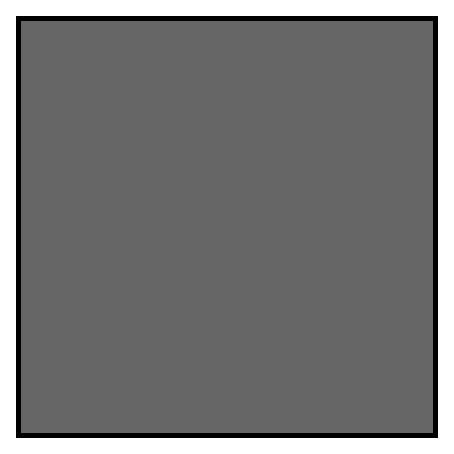
\includegraphics{example.eps}
% figure caption is below the figure
\caption{Please write your figure caption here}
\label{fig:1}       % Give a unique label
\end{figure}
%
% For two-column wide figures use
\begin{figure*}
% Use the relevant command to insert your figure file.
% For example, with the graphicx package use
  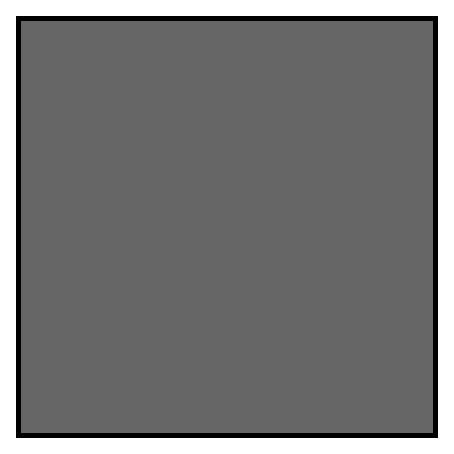
\includegraphics[width=0.75\textwidth]{example.eps}
% figure caption is below the figure
\caption{Please write your figure caption here}
\label{fig:2}       % Give a unique label
\end{figure*}
%
% For tables use
\begin{table}
% table caption is above the table
\caption{Please write your table caption here}
\label{tab:1}       % Give a unique label
% For LaTeX tables use
\begin{tabular}{lll}
\hline\noalign{\smallskip}
first & second & third  \\
\noalign{\smallskip}\hline\noalign{\smallskip}
number & number & number \\
number & number & number \\
\noalign{\smallskip}\hline
\end{tabular}
\end{table}


%\begin{acknowledgements}
%If you'd like to thank anyone, place your comments here
%and remove the percent signs.
%\end{acknowledgements}

% BibTeX users please use one of
%\bibliographystyle{spbasic}      % basic style, author-year citations
%\bibliographystyle{spmpsci}      % mathematics and physical sciences
%\bibliographystyle{spphys}       % APS-like style for physics
%\bibliography{}   % name your BibTeX data base

% Non-BibTeX users please use
\begin{thebibliography}{}
%
% and use \bibitem to create references. Consult the Instructions
% for authors for reference list style.
%
\bibitem{RefJ}
% Format for Journal Reference
Author, Article title, Journal, Volume, page numbers (year)
% Format for books
\bibitem{RefB}
Author, Book title, page numbers. Publisher, place (year)
% etc
\end{thebibliography}

\end{document}
% end of file template.tex

